\documentclass[12pt,a4paper]{article}

\usepackage[utf8]{inputenc}
\usepackage[french]{babel}
\usepackage[T1]{fontenc}
\usepackage{verbatim}
\usepackage{graphicx}
\usepackage{listings}
\usepackage{hyperref}
\usepackage{lmodern}
\usepackage{listings}
\usepackage{textcomp} 
\usepackage{hyperref}
\usepackage{verbatim}

\title{Cahier des charges\\}
\author{Equipe CFR-ESILV 2017\\ [2em]
Paris La Défense\\[2em]
École supérieure d'ingénieurs Léonard-de-Vinci\\[1em]}
\date\today





\newcommand{\latex}{\LaTeX\space}

\begin{document}
\maketitle

\begin{figure}[!h]
\centering

\includegraphics[width=5 cm]{img/Logo_ESILV.jpeg}
\end{figure}

\section{Présentation}

\paragraph{}
Notre équipe pour la Coupe de France de Robotique (CFR) est constituée uniquement d'étudiants de 
l'ESILV (École Supérieure d'Ingénieurs Leonard de Vinci).
Pour bénéficier d'une certaine expérience dans ce projet, sept étudiants de troisième année sont cette année avec nous : 
\paragraph{}
\begin{itemize}
\item POUSSEUR Hugo (chef de projet) 
\item BRINGER Hippolyte
\item FRADET Guillaume
\item HOUAOUI Rabah
\item BOURAGBA Sofiane
\item PIERRE Hugo
\item SAM Medhi 
\end{itemize}



\paragraph{}
Il y a ensuite six étudiants de deuxième année :  

\paragraph{}
\begin{itemize}
\item FONTAINE Nicolas 
\item ISAMBOURG Théo
\item LE LAY Pierre
\item PARILUSYAN Brice
\item PICARD Adrien
\item QUIBEL Florian
\end{itemize}


\paragraph{}
Il y a aussi deux étudiants de troisième année qui sont à l'étranger pendant le premier semestre :

\paragraph{}
\begin{itemize}
\item JONAH HARISON Johan
\item LEMAITRE Corentin
\end{itemize}


\paragraph{}
Un mentor nous a été assigné pour nous suivre tout au long de la réalisation de notre projet : 

\begin{itemize}
\item DJERROUD Halim 
\end{itemize}


\paragraph{}
l'ESILV a déjà participé il y a trois ans, en 2015 et en 2016.
Une association de Robotique "DAVINCIBOT" a d'ailleurs été créée il y a deux ans. 
Nous avons obtenu un statut d'association afin de bénéficier d'aide financière de la part de la 
COFA\footnote{Commission du Financement des Associations} et aussi auprès de sponsors extérieurs. 

\paragraph{}
En effet, la réalisation de robots demande un certain budget pour l'achat des différents composants
(cartes Arduino, cartes Raspberry PI, corps des robots ...).

\paragraph{}
Cette année l'association a changé de bureau : 

Président  : JONAH HARISON Johan 

Trésorier : POUSSEUR Hugo 

\paragraph{}
Guillaume FRADET se charge de la communication web, c'est 
à dire la gestion de notre site, de la page facebook "Davincibot" et du compte 
tweeter "@DavincibotEsilv".

\paragraph{}
Au niveau de l'école, la réalisation de ce projet s'inscrit dans le PIX 2 (Projet d'Imagination
et d'Exploration année 2) et dans le PING (Projet de l'Ingénieur Numérique Généraliste). 
Le but du PIX 2 est : 

\begin{itemize}
\item d'appliquer ce qu'on apprend en cours
\item de travailler en groupe 
\item de découvrir d'autres outils (en plus des cours)
\item de construire un produit 
\item d'apprendre à gerer un long projet avec un budget
\end{itemize}

\paragraph{}
Le but du PING est :

\begin{itemize}
\item Conduire un projet d’envergure et savoir s’adapter
\item Identifier et évaluer les risques
\item Utiliser de nouvelles technologies
\item Se confronter à d’autres
\item Savoir défendre son projet technique
\end{itemize}

\section{Projet}

\subsection{La coupe de France de robotique}

\paragraph{}
La coupe de France de robotique a été créée en 1994 et se déroulait jusqu'en 2014 à la Ferté-Bernard, dans le 
département de la Sarthe. L'année dernière elle a eu lieu à la Roche sur Yon début  mai. Normalement, elle a lieu tous les ans à la fin mai et réunie environ 200 équipes de toute la France 
venues confronter leurs robots sur une table. Le règlement change tous les ans en fonction des épreuves proposées. 
Cette année, le thème est la plage et comporte plusieurs épreuves qui rapportent chacune un nombre de points 
bien définis. Les épreuves se déroulent donc sur une table avec deux concurrents, chacun ayant ces épreuves 
indépendantes de l'autre.  

Ces épreuves sont : 

\paragraph{}
\begin{itemize}
\item Construire des fusées avec des modules lunaire
\item Déposer des modules lunaire et des minerais dans la zone de départ
\item Déposer des minerais dans la soute de sa navette
\item Construire une base lunaire
\item Lancer un engin spatial intégré au robot (Funny Action)
\end{itemize} 

\paragraph{}
Bien sûr, toutes les épreuves ne sont pas obligatoires et peuvent être effectuées dans l'ordre que l'on souhaite  

\subsection{Contraintes à respecter}
\paragraph{}
Il y a donc, comme dans toutes compétitions, des contraintes à respecter. Tout d'abord, un robot ne peut pas 
empêcher l'adversaire de marquer des points, ou gêner de quelconque façons la progression de son adversaire. 
Ensuite vient les contraintes sur le dimensionnement des robots. Le robot principal ne doit pas excéder 1200 
mm de périmètre au départ (donc non déployé), et 1500 mm de périmètre lorsqu'il est déployé. Pour le second 
robot, il ne doit pas dépasser 700 mm au départ et 900 mm déployé. Ils ne doivent pas dépasser 350 mm de hauteur. 
Le robot doit être autonome autant au niveau de sa progression que de son alimentation. 

\paragraph{}
Il doit y avoir deux espaces rectangulaires de 100x70 mm laissés libre sur au moins deux 
faces du robot pour les autocollants de l'organisation.

\paragraph{}
Les robots doivent être démarrés avec un dispositif composé d'un cordon d'au moins 500 mm de long qui ne
restera pas sur le robot après le départ. Ils doivent avoir un bouton d'arrêt d'urgence facilement accessible sur 
le dessus du robot, et aussi d'un système permettant leurs arrêts automatiques au bout de 90 secondes. Ils seront 
composés aussi d'un système permettant d'éviter les autres robots et d'un support pouvant accueillir une balise de détection de l'équipe adverse.

\paragraph{}
Les matchs durent 90 secondes au-delà desquelles les robots ne peuvent plus se déplacer, mais possèdent encore 5 
secondes pour faire la Funny Action. 

\subsection{Épreuves choisies}
\paragraph{}
TOUTE CETTE PARTIE EST A REVOIR !!!!!!!!!!!!!!!!\\ 
Nous avons donc choisi, en fonction de toutes ces contraintes de réaliser les épreuves suivantes : 
\begin{itemize}
\item Drapeaux (10 points par porte)
\item Pêche (5 points hors de l'eau et 10 points dans le filet)
\item Château de sable (2 points par bloc dans la zone, 2 points supplémentaires par bloc empilé et 12 points supplémentaires si le modèle du château est respecté)
\item La Funny Action (20 points si le parasol est valide)
\end{itemize}

\paragraph{}
Nous avons choisi ces épreuves car elles nous paraissent faisables et plutôt facile à réaliser. Pour 
le château de sable nous avons juste décidé de pousser les blocs présents au niveau de la table dans la zone, 
car il y en a en hauteur. Pour les coquillages nous avons décidé que cela allait nous prendre beaucoup de temps à 
réaliser car ils sont de couleurs différentes et certains appartiennent à l'autre équipe. Nous nous sommes dit que 
nous allions prendre trop de risque pour le peu de points que nous pourrions gagner sur cette épreuve. 

\paragraph{}
Nous pensons pouvoir gagner environ 60 à 100 points avec la réalisation de toutes ces épreuves.

\paragraph{}
\begin{tabular}{|l|l|}
  \hline
  Epreuve & Points\\
  \hline
  Module lunaire & 2 par module dans sa zone de départ \\
  Minerai & 2 sur zone et 3 dans la soute \\
	Base lunaire & 10 par module lunaire valide \\
	Funny action & 20 \\
  \hline
\end{tabular}


\subsection{Organisation interne}
\paragraph{}
Pour mener à bien ce projet, nous avons dû nous organiser de manière spécifique. Du fait de la taille de l'équipe. Nous 
utilisons une méthode de travail appelé SCRUM.

Cette méthode de travail inventée en 1986 se base notamment sur des sprints et des "zones critiques".

Elle est très utilisée dans le milieu industriel pour favoriser la vitesse de résolution des différentes étapes, la communication entre l'équipe projet, le client 
et les membres au sein de l'équipe.

\paragraph{}
Cette méthode est bien adaptée à notre situation, nous allons travailler par binômes ou trinômes sur des taches
définies et en évoluant sur les différents postes au sein de l'équipe. Ceci nous permettra de toucher à toutes les facettes du projet,
et d'être au courant de l'avancement de tous les objectifs.\\
Ainsi un membre de l'équipe ne fera pas toujours la même chose et chaque membre apportera sa part à l'ensemble du projet.\\ \\


\paragraph{}
Pour mener à bien ce projet, nous nous organisons comme suit :
\begin{itemize}
\item Une réunion hebdomadaire le lundi après midi 
\item Nous nous voyons aussi en dehors de la réunion du lundi pour pouvoir en faire plus
\item Compte rendu pour chaque réunion
\end{itemize}


\section{Les outils utilisés}

\subsection{Un système d'exploitation pour les robots}

\paragraph{}
Les épreuves que nous devons affronter imposent l'exécution de plusieurs tâches en parallèles, par exemple 
faire avancer le robot tout en ajustant sa position ou tout simplement exécuter différentes tâches
afin de respecter les contraintes temporelles imposées par le règlement. Ce mode de fonctionnement impose une 
programmation parallèles, ce qui n'est pas possible avec les micro contrôleurs de type 
Arduino \footnote{Arduino est un circuit imprimé en matériel libre sur lequel se trouve un micro contrôleur}.
Pour ces raisons nous avons décidé d'utiliser une autre technologie basée aussi sur des micro contrôleurs
plus puissant, à savoir la Raspberry Pi \footnote{Le Raspberry Pi est un nano-ordinateur monocarte à processeur ARM}

\paragraph{}
La programmation parallèle pose à son tour un problème. Il est nécessaire d'avoir
une connaissance approfondie d'un langage de programmation spécialisé tel que C, C++ ou Python. Afin de pallier à ce problème, nous avons 
choisi d'utiliser un système d'exploitation spécialisé dans la programmation des robots. Ce dernier étant conçu dans 
le but de faciliter la programmation des robots. Chaque concepteur de robot passait un temps non négligeable 
à concevoir matériellement son robot ainsi que le logiciel 
embarqué associé. Cela demandait des compétences en mécanique, électronique et programmation embarquée. 
Généralement, les programmes ainsi conçus correspondaient plus à de la programmation embarquée, proche 
de l'électronique, qu'à de la robotique proprement dite, telle que nous pouvons la rencontrer aujourd'hui 
dans la robotique. La réutilisation des programmes était non triviale car fortement liée au 
matériel sous-jacent. 

\paragraph{}
Comme son nom l'indique, ROS (Robot Operating System) est un système d'exploitation pour robots. De même que 
les systèmes d'exploitation pour les ordinateurs. 
Il fournit des services proches d'un système d'exploitation (abstraction du matériel, 
gestion de la concurrence, des processus) mais aussi des fonctionnalités de haut niveau (appels 
asynchrones, appels synchrones, base centralisée de données, système de paramétrage du robot). L'idée principale d'un OS 
robotique est d'éviter de réinventer la roue à chaque fois et de proposer des fonctionnalités standardisées faisant 
abstraction du matériel.

\paragraph{}
Le principe de base d'un OS robotique est de faire fonctionner en parallèle un grand nombre d'exécutables qui 
doivent pouvoir échanger de l'information de manière simple, à l'aide de messages textes. Par exemple,
interroger à une fréquence définie les capteurs du robot (capteur de distance à ultrasons ou infrarouge, capteur 
de pression, capteur de température, gyroscope, accéléromètre, caméras, microphones), récupérer ces informations, 
les traiter (faire ce que l'on appelle la fusion de données), les passer à des algorithmes de traitement (traitement 
de la parole, vision artificielle, localisation et cartographie simultanée) et enfin contrôler les moteurs en retour. 
Tout ce processus s'effectue en continu et en parallèle. D'autre part, l'OS robotique doit assurer la gestion de la 
concurrence afin d'assurer l'accès efficace aux ressources du robot. 


\subsection{Architecture de nos robots}

\paragraph{}
Comme nous l'avons annoncé dès le début de ce rapport nous avons décidé de construire deux robots. Dans le but d'optimiser 
le processus de construction nous avons adopté la même architecture pour les deux robots, nous avons utilisé pour chaque robot 
une carte RaspberryPi2 et une ou plusieurs carte(s) Arduino avec un shield pour contrôler les moteurs qui font avancer le robot.


\begin{figure}[!h]
\centering
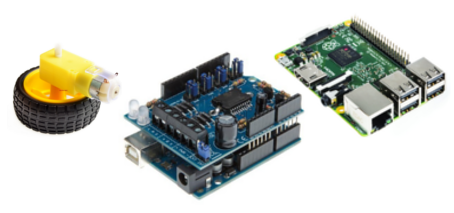
\includegraphics[width=10 cm]{img/img.jpeg}
\caption{RaspberryPi2 , carte Arduino avec un shield et moteur}
\end{figure}

\paragraph{}
Dans la figure suivante nous allons montrer l'architecture générale qui décrit l'agencement des ces différents modules. 
\paragraph{}
Une carte RaspberryPi2 sur laquelle nous avons embarqué l'OS ROS et développé un petit module. Celui-ci permet de contrôler
les moteurs qui font avancer le robot. Cette carte n'est pas assez puissante pour alimenter directement les moteurs, pour cela 
nous avons intercalé entre cette dernière et les moteurs une carte arduino avec un shield prévu pour contrôler les moteurs. 
Sur la carte arduino aussi, un petit code a été embarqué pour communiquer avec la carte RaspberryPi2.
\paragraph{}
Pour les capteurs et les effecteurs qui ne demandent pas une grande quantité d'énergie de fonctionnement nous les avons directement connectés 
sur la carte RaspberryPi2.

\begin{figure}[!h]
\centering
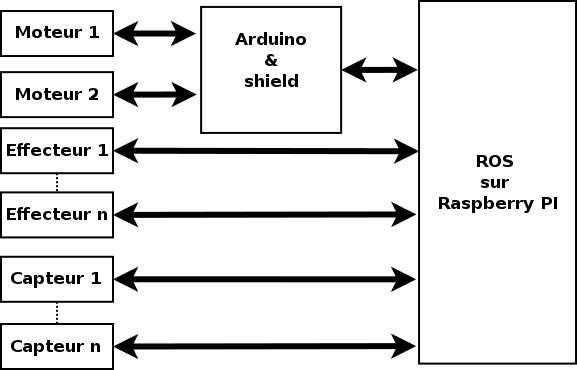
\includegraphics[width=10 cm]{img/archi_1.png}
\caption{Architecture générale}
\end{figure}

\paragraph{}
Pour de valider notre architecture nous avons fait quelques essais avec un petit robot improvisé, ce dernier
a pour but d'interpréter des commandes envoyées par l'utilisateur en utilisant les touches flèches directionnelles du clavier.

\begin{figure}[!h]
\centering
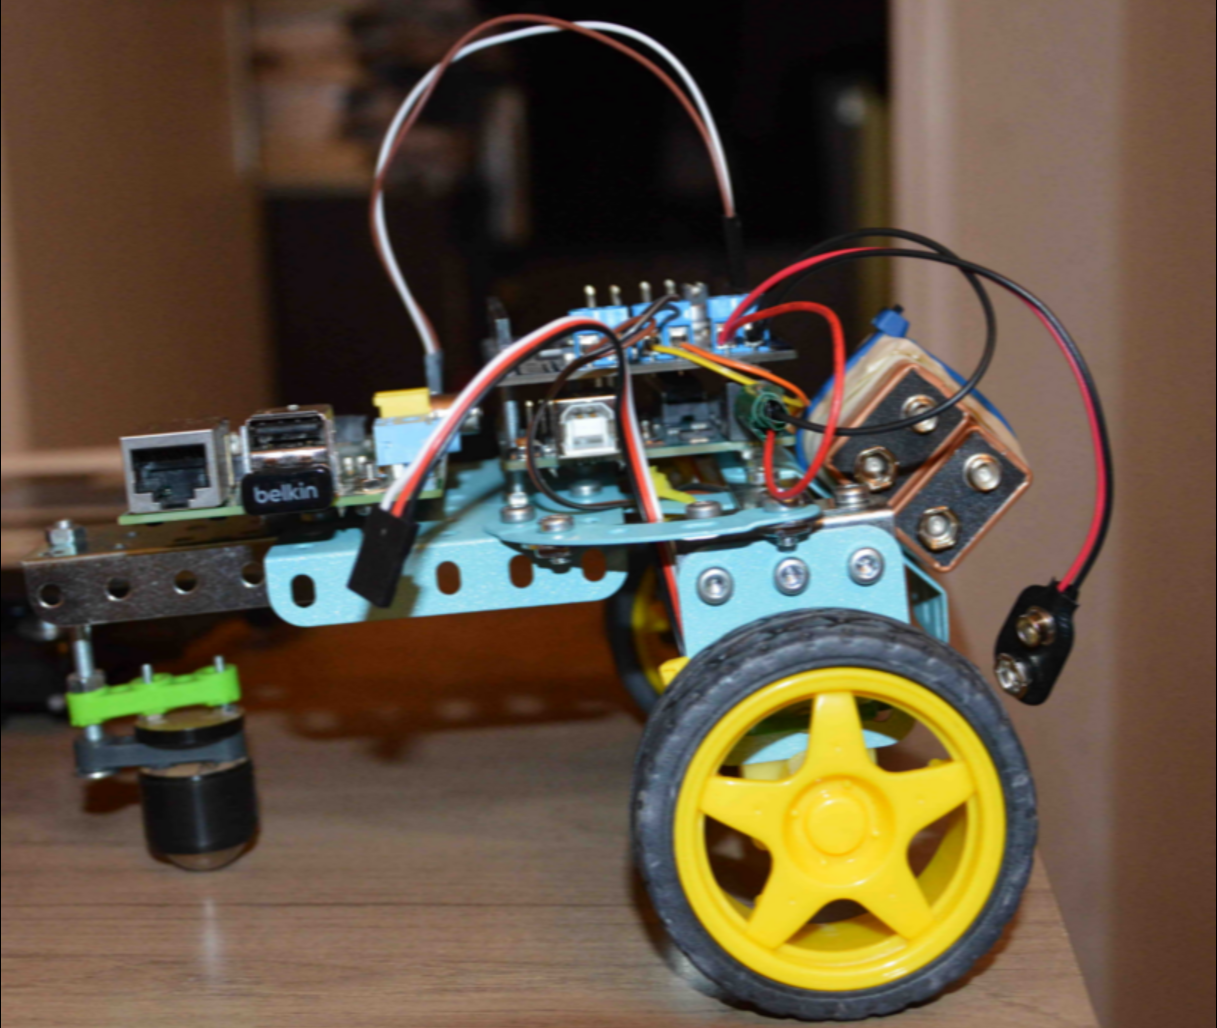
\includegraphics[width=10 cm]{img/robo_test.png}
\caption{tt}
\end{figure}

Le code embarqué sur ROS 

\begin{verbatim}
 
\end{verbatim}

\subsection{La table de jeu}

\paragraph{}
Les deux robots évoluent donc sur une table de jeux possédant des obstacles et des endroits de différentes couleurs. La 
table est de 3000 mm par 2000 mm avec des bordures de chaque côté. Chaque équipe possède une zone de départ matérialisée 
par une zone peinte à la couleur de l'équipe. Toutes les épreuves sont présentes sur la table:  
des drapeaux avec la porte qu'il faut fermer, ensuite les bacs d'eau avec les poissons à pêcher sur le côté de la table. 
Pour le château de sable, il y a une zone où doivent être mis les blocs pour gagner des points. Ces blocs sont éparpillés 
sur l'aire de jeu, avec une place bien définie pour chacun. Ensuite, il y a les coquillages (épreuve que nous 
ne réaliserons pas) qui sont répartis aléatoirement sur la table de jeu, et à des places bien précises sur 
le « rocher ».

\paragraph{}
Nous avons donc décidé de reproduire à l'identique la table pour nous aider dans la réalisation des robots et 
nous permettre de faire des réglages précis.
Pour réaliser notre table, nous possédons déjà la table des années précédentes. Nous allons donc reproduire le 
décor de la table de cette année. Pour se faire nous avons recouvert de papiers adhésifs colorés la table, pour 
ne pas avoir à la peindre. Pour se procurer les différentes pièces nécessaires, la Coupe de France a fourni 
sur son site internet les différents plans des pièces et les fichiers pour les impressions 3D de ces dernières. 
La table sera accessible dans notre salle et nous aider dans la réalisation du robot.


\begin{figure}[!h]
\centering
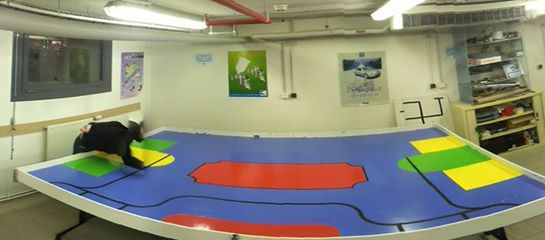
\includegraphics[width=12 cm]{img/table.jpg}
\caption{Table}
\end{figure}


\newpage

\subsection{Un travail collaboratif}

\paragraph{}
Note équipe est composée de quatorze membres, le travail en équipe devient très difficile à partir du moment où on travaille
sur les mêmes tâches. Pour résoudre ce problème épineux, nous avons opté pour 
l'utilisation d'un système de versioning GIT. Ce dernier est un système qui enregistre l'évolution d'un fichier ou d'un 
ensemble de fichiers au cours du temps de manière à ce qu'on puisse rappeler une version antérieure d'un fichier à tout moment.
De plus il permet aussi de gérer les conflits qui peuvent survenir dans le cas où plusieurs utilisateurs travaillent sur 
la même portion de code.

\paragraph{}
Le logiciel git fonctionne en mode décentralisé, c'est-à-dire qu'aucun serveur n'est requis pour fonctionner, mais ce mode 
de fonctionnement est difficile à mettre en place. nous avons opté pour une utilisation du mode centralisé de git, ce mode permet
de centraliser le code sur un serveur et chaque utilisateur pourra consulter et effectuer des modifications. 

\paragraph{}
Nous avons choisi d'utiliser la plate-forme GitHub.
Elle présente l'avantage d'être gratuite et offre une version web qui permet de 
consulter directement les modifications en ligne. Nous avons créé un compte pour chaque membre de l'équipe et nous avons créé 
deux dépôts principaux, le premier permet de gérer nos documents de travail: le planning, le cahier des charges , les documents 
de conception etc. Ces derniers sont consultables sur l'url suivant: 

\paragraph{}
\begin{itemize}
 \item \url{https://github.com/ESCF17/coupe}
\end{itemize}


\subsection{Une documentation de qualité}
\paragraph{}
Afin de produire une documentation de qualité nous avons décidé d'utiliser \LaTeX. 
Beaucoup de personnes se demandent pourquoi nous utilisons un traitement de texte comme LaTeX si 
rébarbatif alors qu'il existe des traitements de texte WYSIWYG \footnote{" what you see is what you get ", signifiant 
littéralement en français " ce que vous voyez est ce que vous obtenez "} de plus en plus performant avec 
des correcteurs orthographiques et grammaticaux, avec création de tableaux par simples clics de souris, 
avec des dizaines de polices de caractères différentes, avec des éditeurs de formules WYSIWYG également.
La réponse est simple \LaTeX  est une vraie merveille si on doit rédiger un document avec de nombreuses pages car la mise 
en forme de celles-ci sont très soignées. De même, la création et la modification de celles-ci sont relativement simple.

\paragraph{}
LaTeX permet à l'utilisateur de se concentrer sur le contenu du document sans se soucier de la mise en forme qui sera 
effectuée automatiquement. Par exemple, on change de taille de caractères relativement à une taille par défaut 
précisée au début du document. Donc si on modifie la taille par défaut, les tailles relatives sont modifiées également 
et il n'est pas nécessaire de mettre à nouveau tout le document en page.

\paragraph{}
Nous avons choisi ce mode d'édition pour l'ensemble de nos document ainsi, d'un coté cela nous permettra 
de nous entraîner à l'utilisation de LaTex et d'un autre coté vu que LaTeX utilise du texte cela 
facilite la rédaction collaborative grâce à Git. 

\subsection{De la conception à la réalisation}
\paragraph{}
Pour la partie conception mécanique nous avons choisi 
le logiciel Solidworks. Il permet de modéliser des objets en 3D. Grâçe au FabLab de l'école, nous allons imprimer 
ces pièces en 3D. Il serait notamment souhaitable d'imprimer la base roulante du robot, et les petits accessoires 
du plateau (les coquillages par exemples...).

\paragraph{}
Solidworks est un logiciel de modélisation, le but de ce logiciel est de
créer des plans de la pièce modélisée. Ces plans peuvent être utilisés par
un centre d'usinage afin de réaliser le produit ou de support pour une
présentation du projet. A l'heure où l'imprimante 3D devient de plus en
plus courante, il est désormais possible d'imprimer directement la pièce à
partir de sa modélisation. Cette technique est intéressante pour la
réalisation de pièces complexes et son faible coût (aucune main
d'œuvre). Nous avons la chance d'avoir accès au FabLab du pôle Léonard de
Vinci composé de plusieurs imprimantes 3D.

\paragraph{}

\begin{figure}[!h]
\centering
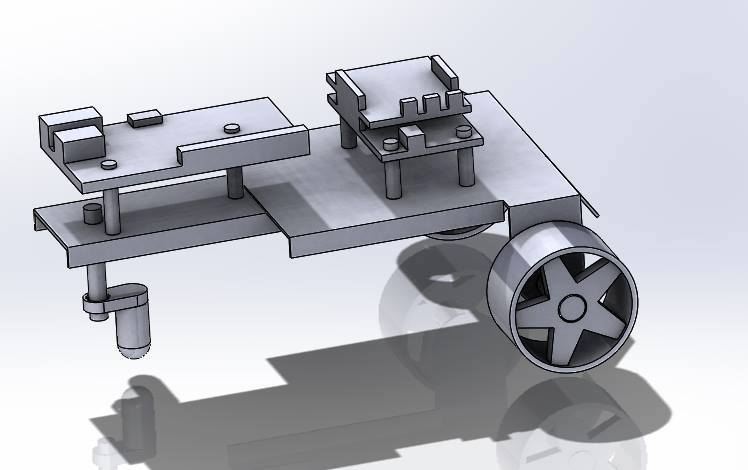
\includegraphics[width=12 cm]{img/robot_con.jpg}
\caption{Robot }
\end{figure}


\section{Calendrier}
\subsection{Date - Coupe de France de Robotique}
\paragraph{}
La Coupe de France de Robotique nous impose quelques deadlines telles que :
\paragraph{}
\begin{itemize}
\item 31/12 : (Deadline) Inscription sur le site Poolzor
	 (http://www.planete-sciences.org/robot/poolzor/)
\item Le 25 mai, qui est le début de la Coupe
\end{itemize}

\subsection{Date - École}
\paragraph{}
La participation à la Coupe de France de Robotique s'inscrit dans le cadre d'un projet donné 
par l'école, de ce fait nous devons respecter plusieurs deadlines qui permettent l'avancement de notre projet :
\paragraph{}
\begin{itemize}
\item 23/11 : Rendu du cahier des charges du projet  (1-2 pages)  +  Définition et répartition des tâches (2-3 pages).
\item 27/11 : Rendu du pitch, filmé (45 à 60 secondes face caméra pour "vendre" notre projet). 
\item 14/12 : Évaluation des membres du projet.
\item 10/01 : Première soutenance (présentation et avancement ).
\item 25/01 : Première commande de matériel.
\item 22/02 : Seconde commande de matériel.
\item 03/04 : Premier prototype.
\item 22/05 : Slides de présentation pour la soutenance finale.
\item 23/05 : Soutenance finale et rendu d'un rapport du projet de 6 à 8 pages .
\item 25/05 : Vidéo projet (1 à 2 minutes) avec un résumé de notre projet, ses avancements et un visuel de nos robots.
\item 01/06 : Journée projets ( présentation  des projets de toutes les équipes).
\end{itemize}


\end{document}